% Estas slides tienen que abrirse con el programa pdfpc que soporta videos embebidos
% el comando es: pdfpc -g slides.pdf
% para los videos se requiere ubuntu-restricted-extras


%\documentclass[compress,handout]{beamer}
\documentclass[compress]{beamer}
% compress pone la seccion abajo de todo
\mode<presentation>


% Theme customization
\usetheme{Copenhagen}
\setbeamertemplate{itemize item}[rectangle] % configure itemize
\setbeamertemplate{itemize subitem}[circle] % configure itemize
\setbeamertemplate{itemize subsubitem}[triangle] % configure itemize
\setbeamertemplate{navigation symbols}{} % remover simbolos de navegacion de las slides
\usefonttheme[onlymath]{serif} % simbolos matematicos en serif (Como es en latex original)

\setbeamertemplate{blocks}[rounded] % blocks corners rounded
\setbeamercolor{block body}{bg=blue!12,fg=black} % color of blocks

% Latex packages
\usepackage{pdfpc-commands} % pdfpc movie commands
\usepackage[utf8]{inputenc}
\usepackage[T1]{fontenc} % para copiar acentos en español del pdf y permite acentos en las notas
\usepackage[spanish]{babel}
\usepackage[binary-units=true,per-mode = symbol]{siunitx} % para manejar las unidades
\usepackage{multirow}
\usepackage{graphicx}
\usepackage{xcolor}
\usepackage{amsmath} % bmatrix
\usepackage[caption=false]{subfig} % caption = false elimina la palabra "Figura" del caption
\setbeamertemplate{caption}{\raggedright\insertcaption\par} % elimina la palabra "Figura" del caption
\usepackage{import} % para el comando import (se usa para pdf_tex)
\captionsetup[subfigure]{labelformat=empty} % remover el indice del caption de la subfigura
\usepackage{booktabs} % \toprule \midrule \bottomrule
\usepackage[overridenote]{pdfpc} % requires to download manually pdfpc.sty package from https://www.ctan.org/pkg/pdfpc
\usepackage[backend=biber]{biblatex} % set biber to format references. Must configure Biber in Texstudio

% Color commands for annotations
\newcommand\TODO[1]{\textbf{\textcolor{red}{#1}}} %  TODO notes

% add bibliography resource
\renewcommand*{\bibfont}{\footnotesize} % change bibliograhy size
\bibliography{./src/bibliography.bib}


% add math preamble
%\usepackage{amsmath}
\usepackage{amssymb}
\usepackage{amsopn}
\usepackage{mathtools}

% math
\renewcommand{\vec}[1]{\boldsymbol{\mathbf{#1}}}
\newcommand{\norm}[1]{\lVert#1\rVert}

% Declare arg max and arg min functionss
\DeclareMathOperator*{\argmax}{arg\,max}
\DeclareMathOperator*{\argmin}{arg\,min}

% Homogeneous decoration function
\newcommand{\homo}[1]{\dot{#1}}


% Declare projection as math function
\DeclareMathOperator{\proj}{proj}
\newcommand{\fromCoord}[2]{{#1}_\mathrm{#2}}
\newcommand{\toCoord}[2]{\prescript{\mathrm{#2}}{}{#1}}
\newcommand{\worldCoordSystem}{\mathrm{w}}
\newcommand{\bodyCoordSystem}{\mathrm{B}}
\newcommand{\cameraCoordSystem}{\mathrm{c}}
\newcommand{\point}{\vec{p}}
\newcommand{\worldPoint}{\toCoord{\point}{\worldCoordSystem}}
\newcommand{\imagePoint}{\vec{u}}
\newcommand{\cameraPoint}{\toCoord{\point}{\cameraCoordSystem}}
\newcommand{\homoWorldPoint}{\toCoord{\homo{\point}}{\worldCoordSystem}}
\newcommand{\homoImagePoint}{\homo{\imagePoint}}
\newcommand{\homoCameraPoint}{\toCoord{\homo{\point}}{\cameraCoordSystem}}
\newcommand{\measurement}{\vec{z}}
\newcommand{\prediction}{\hat{\vec{z}}}
\newcommand{\seMatrix}{\vec{\xi}}
\newcommand{\transform}[2]{\toCoord{\fromCoord{\seMatrix}{#2}}{#1}}
\newcommand{\pointCoord}[1]{\toCoord{\point}{#1}}
\newcommand{\rotation}{\vec{R}}
\newcommand{\rotationCoord}[2]{\toCoord{\fromCoord{\rotation}{#2}}{#1}}
\newcommand{\translation}{\vec{t}}
\newcommand{\translationCoord}[2]{\toCoord{\fromCoord{\translation}{#2}}{#1}}
\newcommand{\intrinsicMatrix}{\vec{K}}
\newcommand{\principalPoint}{\vec{c}}
\newcommand{\reprojectionError}{u}
\newcommand{\projectionMatrix}{\vec{P}}
\newcommand{\cameraCenter}{\vec{o}}
\newcommand{\essentialMatrix}{\vec{E}}
\newcommand{\inverse}[1]{{#1}^{-1}}

% Motion model
\newcommand{\position}{\vec{p}}
\newcommand{\orientationQuaternion}{\vec{q}}
\newcommand{\predictedPosition}{\hat{\vec{p}}}
\newcommand{\predictedOrientationQuaternion}{\hat{\vec{q}}}
\newcommand{\linearVelocity}{\vec{v}}
\newcommand{\angularVelocity}{\vec{\omega}}

\DeclareMathOperator{\slerpOp}{slerp}
\newcommand{\slerp}[1]{\slerpOp{\left( #1 \right)}}

% Map structure
\newcommand{\map}{M}
\newcommand{\keyframesSet}{K}
\newcommand{\mapPointsSet}{P}
\newcommand{\observedMapPoints}{O}
\newcommand{\covisibilityKeyframes}{CK}
\newcommand{\localMap}{local\_map}



% Bundle Adjutment
\newcommand{\update}{\vec{\delta}}
\newcommand{\incremental}{\hat{\update}}


% Loop Closure names

% scaled operators and letters to fancy view
\newcommand{\sminus}{\scalebox{0.5}[1.0]{$-$}}
\newcommand{\splus}{\scalebox{0.6}[0.6]{$+$}}
\newcommand{\curr}{c}
\newcommand{\sind}[1]{\scalebox{0.6}[0.6]{$#1$}}
\newcommand{\ind}[1]{\scalebox{0.7}[0.7]{$#1$}}

\newcommand{\keyframe}{\vec{K}}
\newcommand{\bowVector}{\vec{v}}
\newcommand{\lcError}{\vec{\Omega}}
\newcommand{\relativeTransformation}{\seMatrix}
\DeclareMathOperator{\interpolate}{interpolate}

\newcommand{\relativeMotion}{\vec{\delta}}
\newcommand{\groundTruth}[1]{{#1}^{*}}



% definición del operador rot()
\DeclareMathOperator{\rotationOp}{rot}
\newcommand{\getRotation}[1]{\rotationOp{\left( #1 \right)}}

\DeclareMathOperator{\translationOp}{trans}
\newcommand{\getTranslation}[1]{\translationOp{\left( #1 \right)}}









\title{Robótica Móvil}
\author{}
\institute{Universidad Nacional de Rosario}
%\date{\scriptsize{Julio 1, 2021}}
\date{}

\begin{document}

% add title page
\frame{\titlepage}


\section{Organización de la Materia}
\begin{frame}
    \frametitle{Organización de la materia}

\end{frame}

\section{Introducción}
\begin{frame}
	\frametitle{Robots de ficción}
     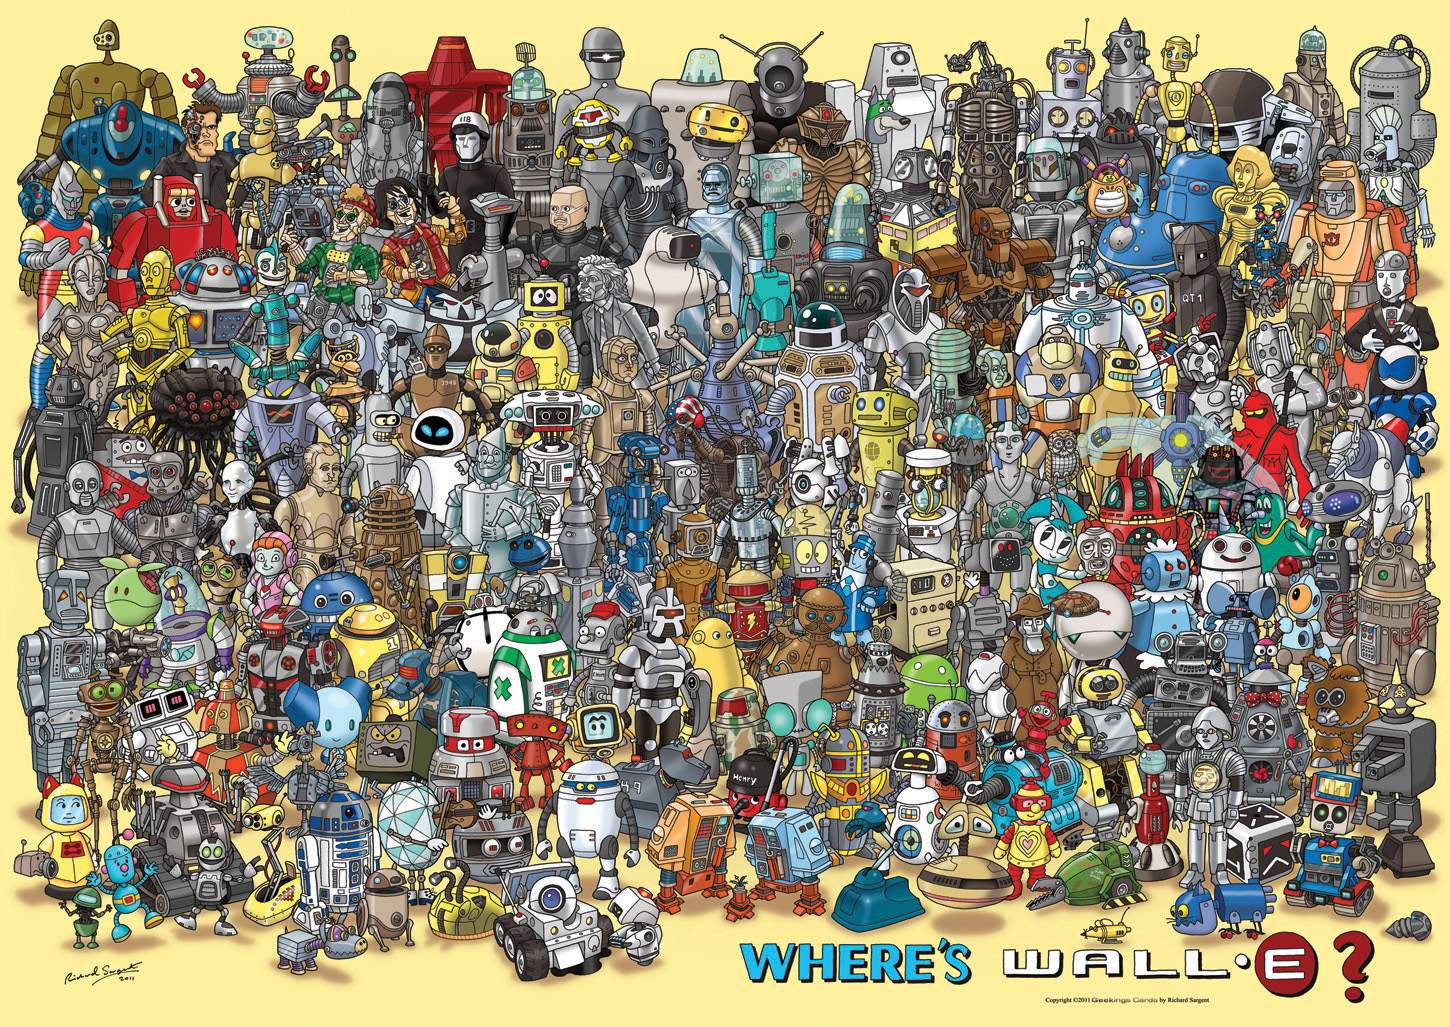
\includegraphics[width=\columnwidth]{wheres_wall_e_poster.jpg}
\end{frame}

\begin{frame}
    \frametitle{Un poco de Historia}
    
    La primera aparición de la palabra robot es utilizada por Karl Capek en 1921 en su obra teatral R. U. R. (Rossumovi Univerzální Roboti Rossum's Universal Robots). La palabra robot viene de la palabra checa \emph{robota} que significa esclavo.
    
    
    \centering
    \begin{figure}
    	\subfloat[]
    	{
    		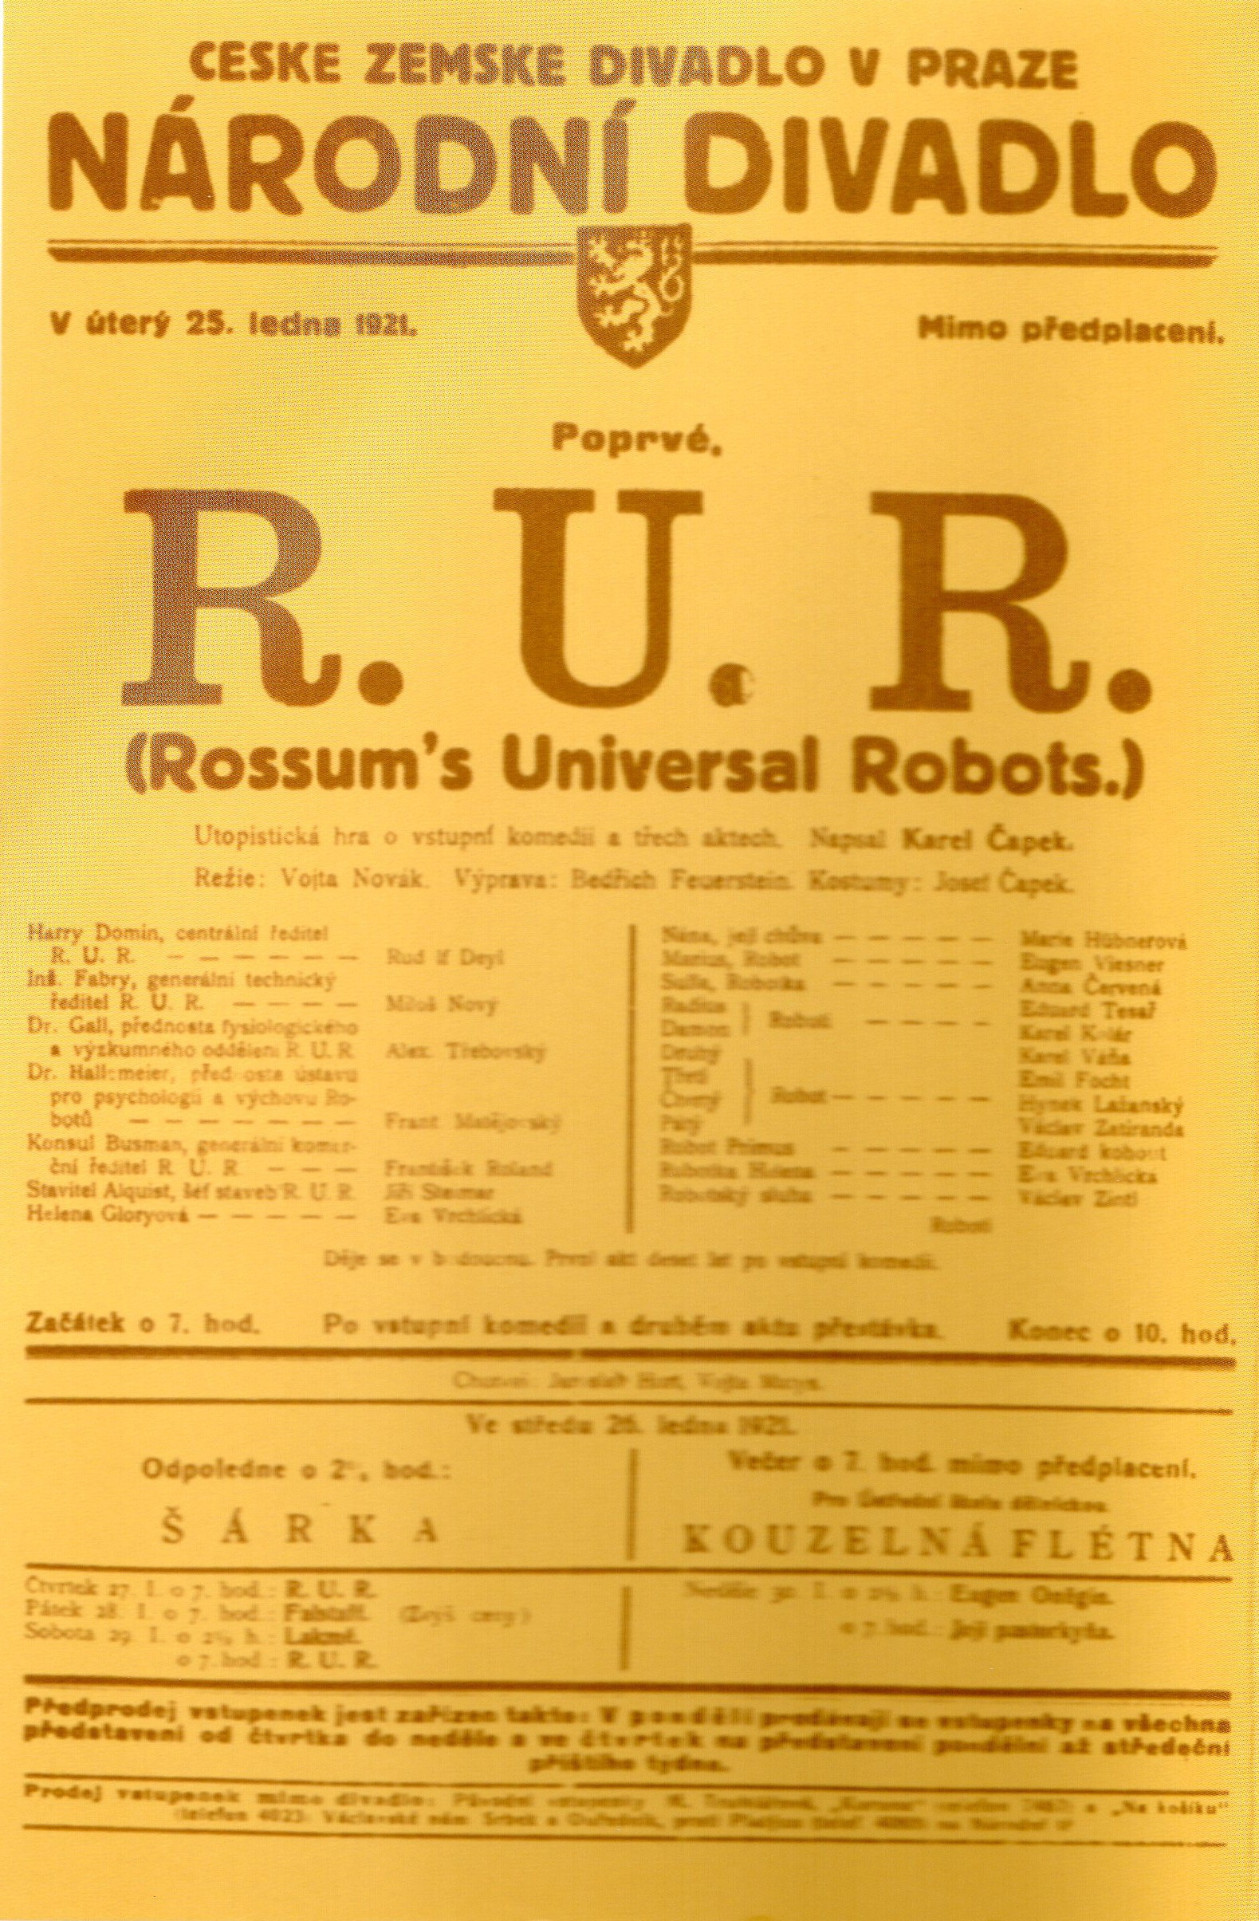
\includegraphics[width=0.2\columnwidth]{rossums_universal_robots_poster.jpg}
    	}\hfill
    	\subfloat[]
    	{
   			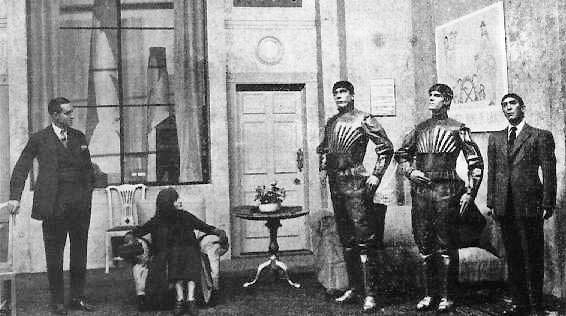
\includegraphics[width=0.5\columnwidth]{rossums_universal_robots_play.jpg}
    	}
    \end{figure}
    
    \note{
        Fuente: https://cs.stanford.edu/people/eroberts/courses/soco/projects/1998-99/robotics/history.html\\
        La obra teatral trata sobre una empresa que construye humanos artificiales orgánicos con el fin de aligerar la carga de trabajo del resto de personas. Aunque en la obra a estos hombres artificiales se les llama robots, tienen más que ver con el concepto moderno de androide o clon. Se trata de criaturas que pueden hacerse pasar por humanos y que tienen el don de poder pensar. Pese a ser creadas para ayudar a la humanidad, más adelante estas máquinas entrarán en confrontación con la sociedad, iniciando una revolución que acabará destruyendo la humanidad.}
\end{frame}

\begin{frame}
    \frametitle{Un poco de Historia}
    
    La palabra \emph{robotics} también fue utilizada por primera vez por Issac Asimov en 1942 en su cuento corto \emph{Runaround} (en español Circuito Vicioso).

    \begin{itemize}
        \item Primera Ley: Un robot no hará daño a un ser humano ni, por inacción, permitirá que un ser humano sufra daño.
        \item Segunda Ley: Un robot debe cumplir las órdenes dadas por los seres humanos, a excepción de aquellas que entren en conflicto con la primera ley.
        \item Tercera Ley: Un robot debe proteger su propia existencia en la medida en que esta protección no entre en conflicto con la primera o con la segunda ley.
    \end{itemize}

    
    \note{The word robotics was also coined by a writer.  Russian-born American science-fiction writer Isaac Asimov first used the word in 1942 in his short story Runabout.  Asimov had a much brighter and more optimistic opinion of the robot's role in human society than did Capek.  He generally characterized the robots in his short stories as helpful servants of man and viewed robots as a better, cleaner race.  Asimov also proposed three "Laws of Robotics" that his robots, as well as sci-fi robotic characters of many other stories.}
\end{frame}

\begin{frame}
    \frametitle{¿Qué es un Robot?}
   
    \begin{block}{Según Robot Institute of America, 1979}
        Un manipulador reprogramable y multifuncional diseñado para mover material, piezas, herramientas o dispositivos especializados a través de varios movimientos programados para el desempeño de una variedad de tareas.
    \end{block}
    
    \begin{block}{Según la RAE}
        Máquina o ingenio electrónico programable que es capaz de manipular objetos y realizar diversas operaciones.
    \end{block}
    
    \begin{block}{Una definición que usamos (\url{https://robots.ieee.org/learn/what-is-a-robot/}):}
        Un robot es una máquina autónoma capaz de sensar su entorno, realizar cálculos para tomar decisiones y realizar acciones en el mundo real.
    \end{block}
    
    \note{hay varias definiciones.\\
    Fuente: https://robots.ieee.org/learn/what-is-a-robot/}
\end{frame}

\begin{frame}
    \frametitle{Shakey the robot: el primer robot móvil autónomo}
    
   
    \begin{columns}[T] % align columns
        \begin{column}{.4\textwidth}
            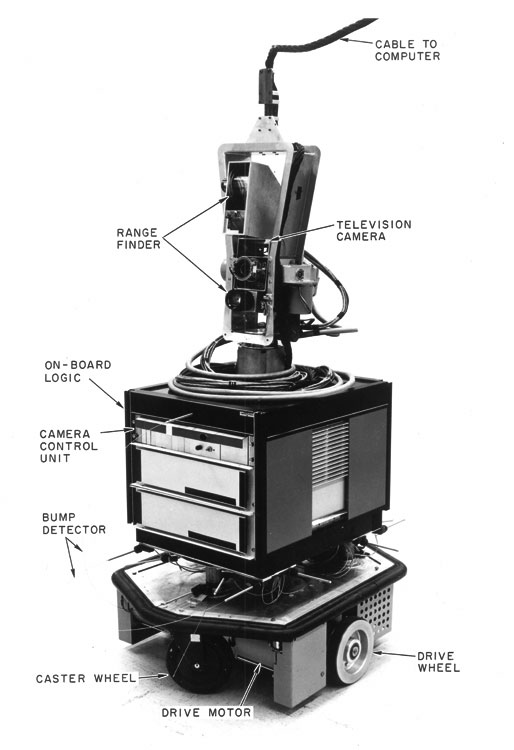
\includegraphics[width=\columnwidth]{shakey.png}
        \end{column}%
        \hfill%
        \begin{column}{.56\textwidth}
              Desarrollado durante 1966 - 1972 por Stanford Research Institute International (SRI).
              
              Resultados: A*, Hough transform y visibility graph.
              
        \end{column}%
    \end{columns}

    \note{Fueten: Wikipedia\\
        Shakey experienced a limited world. A version of Shakey's world could contain a number of rooms connected by corridors, with doors and light switches available for the robot to interact with.\\
        The development of Shakey had a far-reaching impact on the fields of robotics and artificial intelligence, as well as computer science in general. Some of the more notable results include the development of the A* search algorithm, which is widely used in pathfinding and graph traversal, the process of plotting an efficiently traversable path between points; the Hough transform, which is a feature extraction technique used in image analysis, computer vision, and digital image processing; and the visibility graph method for finding Euclidean shortest paths among obstacles in the plane\\
        An example mission for Shakey might be something like:\\
        An operator types the command push the block off the platform at a computer console. Shakey looks around, identifies a platform with a block on it, and locates a ramp in order to reach the platform. Shakey then pushes the ramp over to the platform, rolls up the ramp onto the platform, and pushes the block off the platform. Mission accomplished.}
\end{frame}

\begin{frame}
    \frametitle{¿Qué es la Robótica?}
    La robótica es la intersección de la ciencia, la ingeniería y la tecnología que produce máquinas, llamadas robots, que sustituyen (o replican) las acciones humanas.
\end{frame}

\begin{frame}
    \frametitle{Aplicaciones de la Robótica}
    
    \note{https://robots.ieee.org/learn/types-of-robots/}
    
	\begin{figure}[!h]
        \centering
        \subfloat[] 
        {
            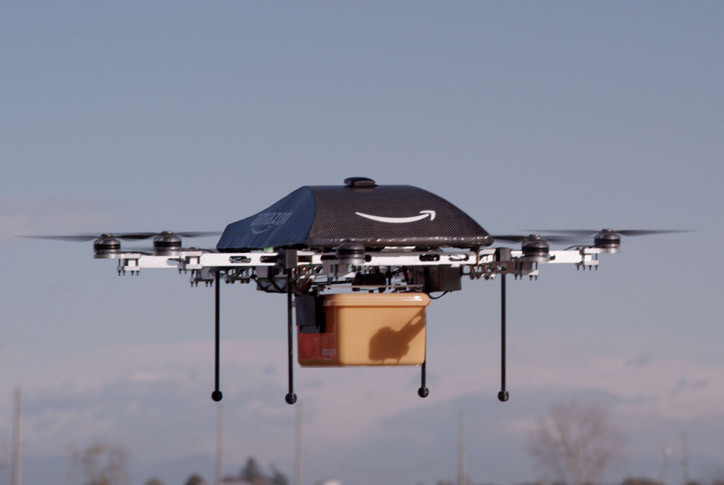
\includegraphics[width=0.33\columnwidth]{./images/drone.jpg}
        }
        \subfloat[] 
        {
            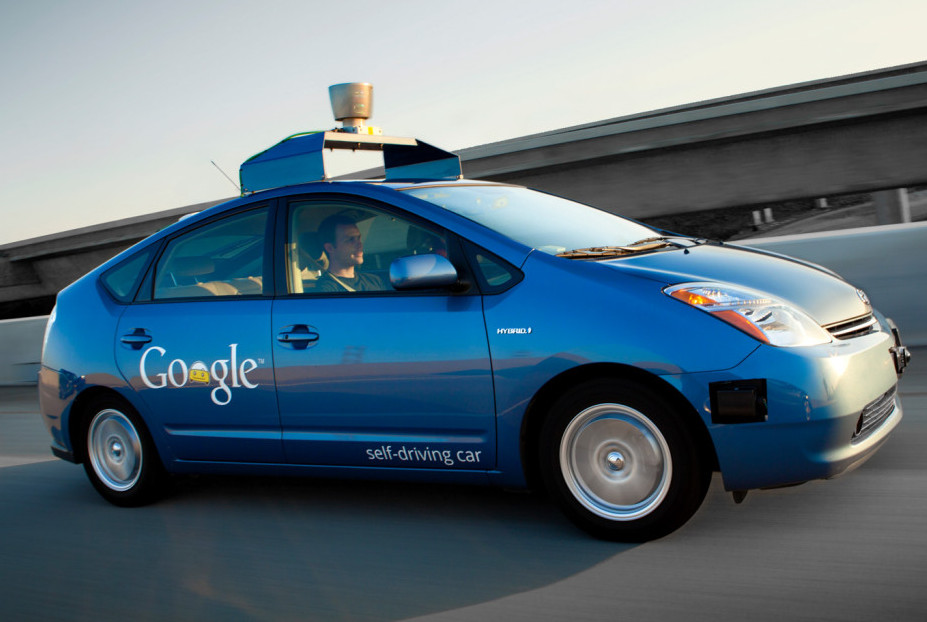
\includegraphics[width=0.33\columnwidth]{./images/google_car.jpg}
        }
        \subfloat[] 
        {
            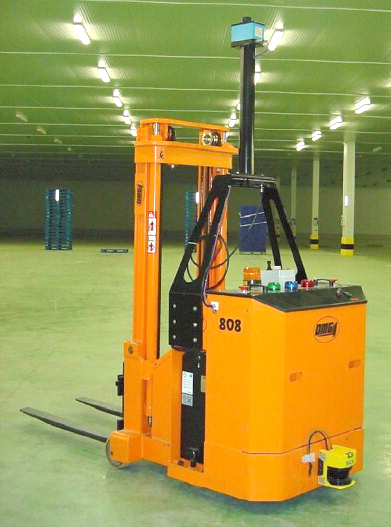
\includegraphics[width=0.16\columnwidth]{./images/industrial_robot.png}
        }\\
        \subfloat[] 
        {
            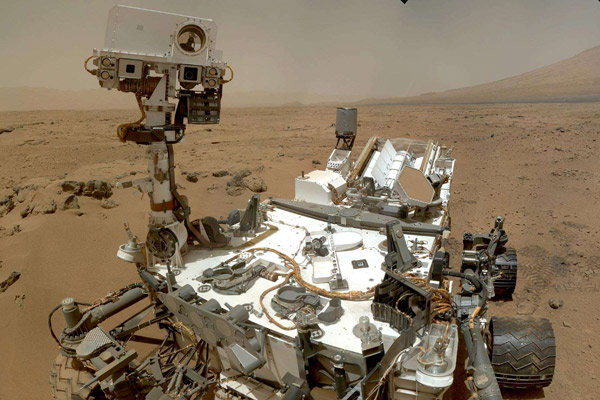
\includegraphics[width=0.33\columnwidth]{./images/curiosity.png}
        }
        \subfloat[] 
        {
            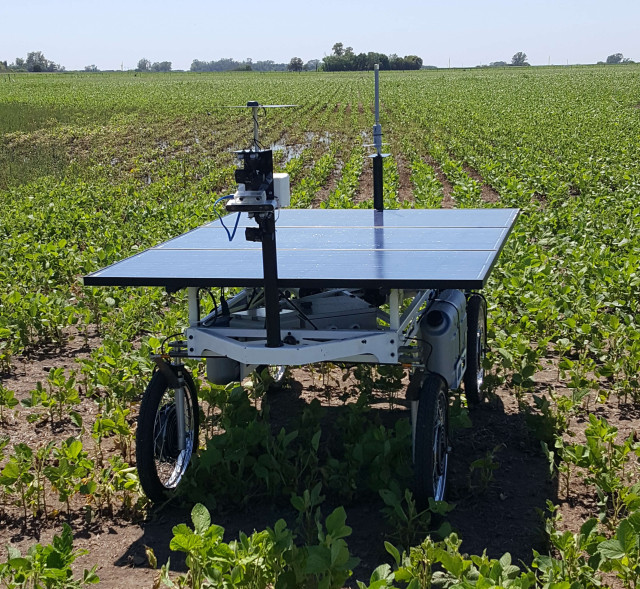
\includegraphics[width=0.27\columnwidth]{./images/weed_removal_robot.jpg}
        }
        \subfloat[]
        {
            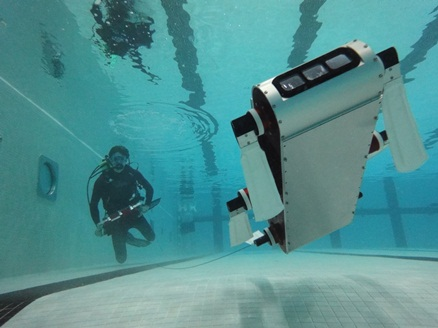
\includegraphics[width=0.3\columnwidth]{./images/aqua.png}
        }		 
    \end{figure}
\end{frame}

\begin{frame}
    \frametitle{Aplicaciones de la Robótica}

    \begin{columns}[T] % align columns
        \begin{column}{.48\textwidth}
            \begin{itemize}
                \item Vehículos autónomos
                \item Industriales 
                \item Cuidado de la Salud
                \item Aeroespacial
                \item Robots de consumo
                \item Respuesta a desastres/catástrofes
                \item Drones (UAV)
            \end{itemize}
        \end{column}%
        \hfill%
        \begin{column}{.48\textwidth}
            \begin{itemize}
                \item Educación
                \item Entretenimiento
                \item Exoesqueletos
                \item Humanoides
                \item Militares
                \item Investigación
                \item Telepresencia
                \item Submarinos
            \end{itemize}
        \end{column}%
    \end{columns}

\end{frame}

\begin{frame}
    \frametitle{Tipos de Robots según locomoción o entorno}
    
    Brazos robóticos
    Robots con patas
    Robots acuáticos
    Robots Humanoides
    Robots aéreos
    
\end{frame}


\begin{frame}
    \frametitle{Navegación autónoma}
    \begin{block}{}
        La navegación autónoma puede definirse a grandes rasgos como la capacidad de moverse de forma segura a lo largo de una trayectoria entre un punto de inicio y uno final [1].
    \end{block}
    \vspace{5mm}
    \begin{columns}
        \column{0.4\textwidth}
        \hspace{13pt}Pregunta:
        \begin{enumerate}
            \visible<2-7>{ \item[-] ¿Dónde estoy?}
            \visible<4-7>{\item[-] ¿Por dónde estoy yendo?}
            \visible<6-7>{\item[-] ¿Cómo llego hasta allí?}
        \end{enumerate}
        \column{0.6\textwidth}
        Respuesta:
        \begin{enumerate}[$\rightarrow$]
            \visible<3-7>{ \item  Cálculo de la posición (Localization)}
            \visible<5-7>{ \item  Representación del entorno (Mapping)}
            \visible<7-7>{\item  Planeamiento de movimiento (Motion planning)}
        \end{enumerate}
    \end{columns}
    \only<4>{}
    \vfill
    \begin{tiny}
        [1] J. J. Leonard - et al., ``Mobile robot localization by ...,'' IEEE Transactions on Robotics and Automation, 2002.
    \end{tiny}
\end{frame}


\begin{frame}
    \frametitle{Estado del arte}
    
    

    \TODO{Comentar los problemas actuales del estado del arte. Lor problemas al trabajr con sensores que tienen error, dependiendo el entorno y la aplicación que tiene que hacer el robot hay que resolver diferentes problemas. Dar ejemplos, problemas que hay en el agua, en outdoor con la luz, de noche, blur, comentar problemas con las camaras,}
\end{frame}

\section{Bibliografía}
\begin{frame}
	\frametitle{Bibliografía}
	
	Capítulo 3 y 7 de: \cite{thrun2005probabilistic}
	
	Shon and Lindsen: Manipulating the Multivariate Gaussian Density
	
	\printbibliography
	
\end{frame}

\end{document}
